\documentclass[12pt, letterpaper]{article}

\usepackage{color} %% Allows text to be typeset in color.

%% These allow Me to add Images to the Book.
\usepackage{graphicx}
\graphicspath{ {images/} }

%% Enables hyperlinks.
\usepackage{hyperref}

%% Makes BigO easier.
\newcommand{\bigO}{\mathcal{O}}
\newcommand{\bigOmega}{\Omega}
\newcommand{\bigTheta}{\Theta}

%%
\oddsidemargin0cm
\evensidemargin0cm
\topmargin-2cm     % These lines increase the amount of usable space and save trees.
\textwidth16.5cm
\textheight23.5cm  

%%\setcounter{tocdepth}{4} %% set the table of contents detail depth.

%% Types of organizational sections.s
%%\part{}
%%\chapter{}
%%\section{}
%%\subsection{}
%%\subsubsection{}
%%\paragraph{}
%%\subparagraph{}

\begin{document}

\title{\color{blue}2D Rendering Assignment v1.0}
\author{Written by Bryce Summers \texttt(BryceSummers.com)}
\date{\color{red}Last Updated: \today}
\maketitle

\tableofcontents 

\section{Overview}

This assignment runs the gauntlet of common Rendering Techniques. The student will learn about explicit function based forms, implicit paramaterization based forms, coordinate space transformations, Function Scaling, color interpolation, Sampling, antialiasing, bounding boxes, 2D renderer implementation, Optimized Super Sampler implementation.

\section{Basic Renderer Setup}

\subsection{Color Calculation functions}
All images can be thought of as a color intensity function on a restricted rectangular domain that takes 2 arguments and returns a color. Many people view images as collections of pixels, but it is usuful to not be restricted by this world view, because often the mathematical specification for an image transcends a given rendering of the image.

\subsection{Rendering}
Rendering is the proccess of converting a mathematical description of a scene into an image.

The standard rendering algorithm is as follows for scenes defined by Color Calculation functions:
\begin{verbatim}
image = Color[h][w];
CCF = [Scene Description Function]

for(int y = 0; y < h; y++)
for(int x = 0; x < w;x++)
{
   image[y][x] = CCF.getColor(x, y);
}
\end{verbatim}

\subsection{Task 1: Implement A Basic Renderer}

\subsection{Optimized Super Sampling}

Super Sampling is the proccess of sampling the color calculation function more than once for a pixel and averaging the results in order to eliminate aliasing in the final image do to defficiencies in the closeness of the sampled pixels.

\begin{verbatim}

image;// Already Rendered using standard rendering.

for(int y = 0; y < h; y++)
for(int x = 0; x < w;x++)
{
   if(pixel differs from a neighboring pixel)
   {
      Color c = average color for all of the sub samples.
      image[y][x] = c;	
   }
}
\end{verbatim}

\subsection{Task 2: Implement an Optimized Super Sampler.}

\newpage
\section{Implicit Rendering: Mandelbrot Set}

\begin{center}
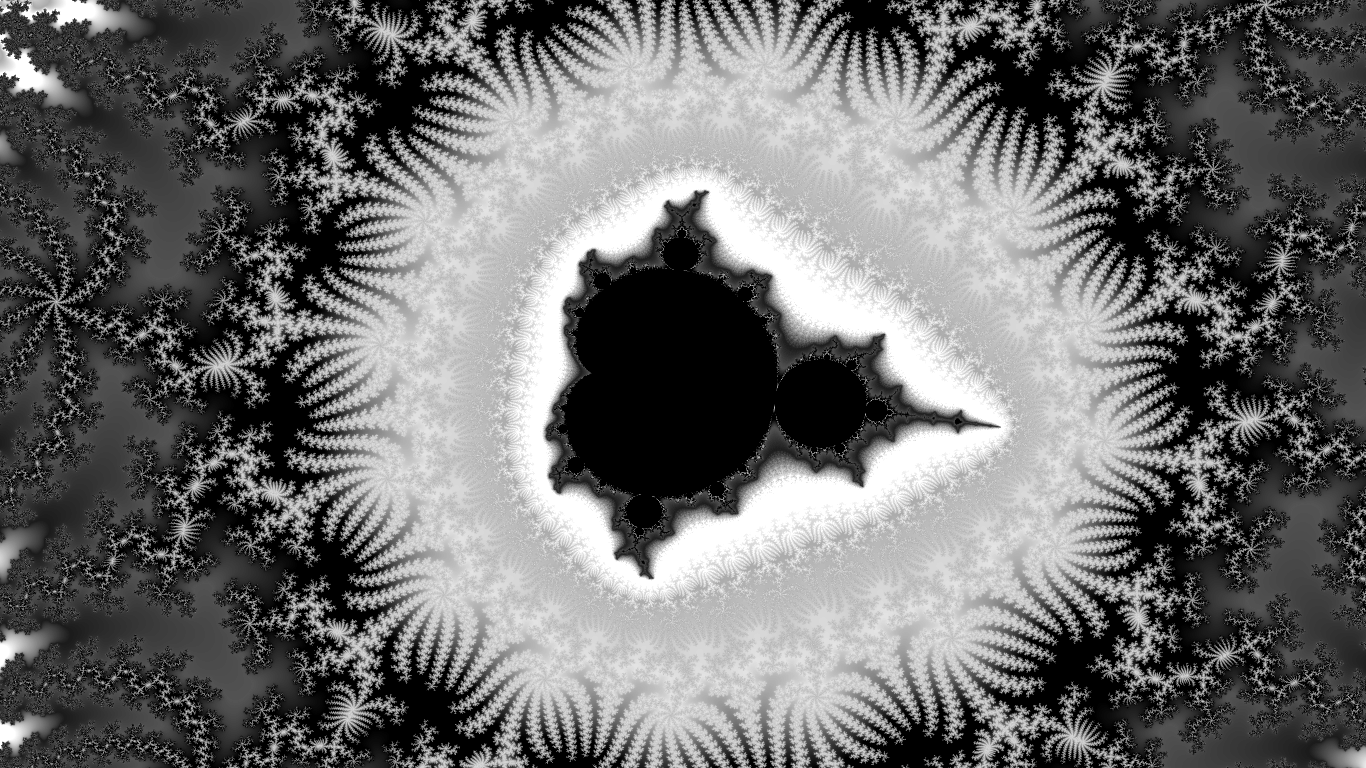
\includegraphics[width=0.5\textwidth]{Mandelbrot.png}
\end{center}

\subsection{Color Calculation Function}
Create the Color calculation function for the Mandelbrot set with a view from (x1, x2) to (y1, y2).

// FIXME Elaborate on the Mandelbrot Generative Procedure.

\begin{enumerate}
\item Input x, y;
\item Transform (x,y) from screen space to fractal space.
\item Apply Iterative Mandelbrot Formula to the point until it excapes the unitary complex circle or it hits the iteration limit.
\item Compute a distance estimation value and apply an interpolation function to produce a nice pallet of colors.
\item Return the final color.
\end{enumerate}

\subsection{Task 3: Mandelbrot Rendering}

Render the appropiate test scenes using super sampling. Make sure you use the optimization so that you do not spend too much of the computation time on the large bodies of set interior points.

\newpage
\section{Explicit Rendering: Barnsley Fern}

\begin{center}

\includegraphics[width=0.5\textwidth]{Fern.png}
\end{center}

Create the Color calculation function for the Barnsley Fern.

\subsection{Precomputations}
Fractal Space:

$$-2.1820 < x < 2.6558 \; \textbf{and} \; 0 \le y < 9.9983$$

We will store irradiance values for every pixel in the image. $\bigO(ITERATIONS)$
We will do a precomputation where we will generate irradiance values for a point traveling according to the Barnsley Fern iterative generation function.

The irradiance points will always hit 4 pixels at a time. The relative additive contributions should be determined by the fractional componant of the floating point location. The location the values are stored at will need to be determined by transforming the location from fractal space to screen space.

We will then do a precomputation where we compute the distance every point is from the fractal. This requires a breadth first search like specialized algorithm form propogating the chaotic values. It also requires a Queue. $~\bigO(PIXELS)$

Compute the Maximum irradiance in order to scale the values appropriately.

// FIXME Elaborate on the math for the generative procedure.

\subsection{Color Calculation Function}

Using the procomputed data, we will specify the Color Calculation Function as follows:

\begin{enumerate}
\item Input x, y;
\item Transform (x,y) from screen space to fractal space.
\item Shade according to the precomputed distance estimation function if the point is not in the fractal. Shade according to the irradiance value relative to the maximum irradiance value otherwise.
\item Return the final color.
\end{enumerate}

Please note that their is no need for super sampling, because the fast changing parts of the signal have already been interpolated in the precomputation step.

\subsection{Task 4: Render The Barnsley Fern}


\section{Piesewise Rendering: Geometric Shapes}

\begin{figure}[h]
\centering

\includegraphics[width=0.5\textwidth]{RenderedText.png}
\caption{Example Text written in Bryce Font 2, which is made out of circles, lines, and locus curves.}
\label{fig:Sub-Line}
\end{figure}

// FIXME : Expand on the transformation math required to properly define these shapes.

\subsection{Circles}

\begin{center}
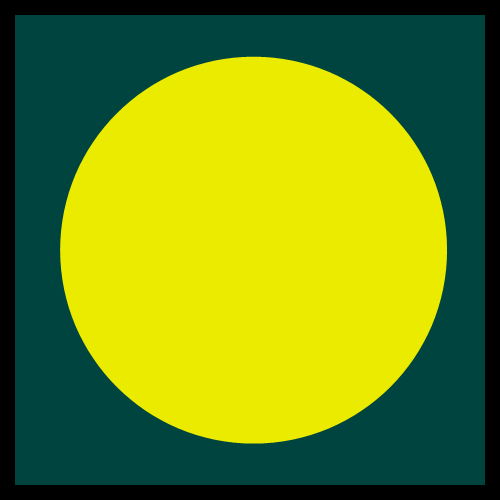
\includegraphics[width=0.25\textwidth]{Circle.png}
\end{center}

The region withing a bounded distance from a central point.

\subsection{Lines}

\begin{center}

\includegraphics[width=0.25\textwidth]{Lines.png}
\end{center}

The region defined by two points that is of a given stroke size perpendicular to the direction specified by the difference between the two points.

\newpage
\subsection{Subdivision Curves}

\begin{center}

\includegraphics[width=0.19\textwidth]{SubLine.png}
\end{center}

Defined by the subdivision of a polyline.

\subsection{Locus Curves}

\begin{center}

\includegraphics[width=0.25\textwidth]{LocusCurve.png}
\end{center}

The portion of a circle that goes through 3 points.

//FIXME : Write up my nifty line side inclusion / exclusion algorithm for explicitly checking for inclusion in theis shape.


\begin{figure}[h]
\centering

\includegraphics[width=0.19\textwidth]{SubLine0.png}

\includegraphics[width=0.19\textwidth]{SubLine1.png}

\includegraphics[width=0.19\textwidth]{SubLine2.png}

\includegraphics[width=0.19\textwidth]{SubLine3.png}

\includegraphics[width=0.19\textwidth]{SubLine4.png}
\caption{A 2D polyLine being subdivided into an interpolated curve.}
\label{fig:Sub-Line}
\end{figure}


\subsection{Task}

Render the test scenes that specify geometry of the forms discussed earlier in this section.
Invent the specification for forms that represent one of the letters of the alphabet.

// Notes: we may want to have the shapes define interpolated in boundedness functions. We could also have people get some hands on experience with alpha blending. We might also want to include some data structures such as bounding boxes to make this task go better.

\subsection{Submission}

There is no submission procedure as of yet.

\subsection{Starter Code}

There is no starter code as of yet.

%% Signals that the document has ended.
\end{document}